\documentclass[tikz,border=2mm]{standalone}
\usepackage{palatino}
\usepackage{tikz}
\usetikzlibrary {shapes.geometric}

\begin{document}

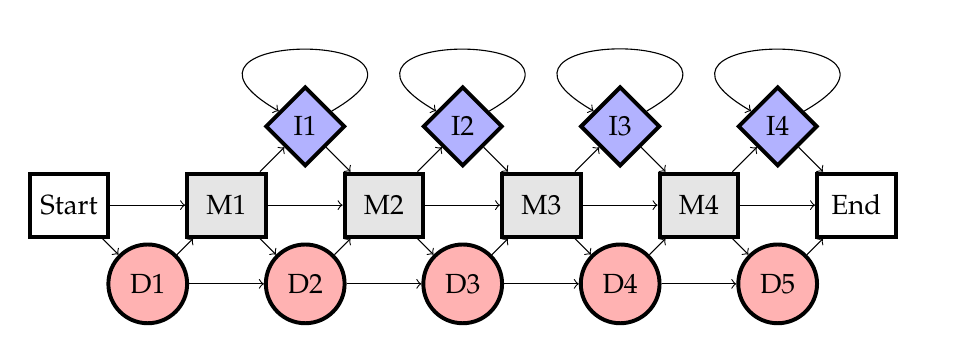
\begin{tikzpicture}
% Define the node styles
\tikzstyle{state} = [draw, minimum width=1.cm, minimum height=0.8cm, line width = .05cm,]
\tikzstyle{match} = [state, rectangle, fill=gray!20]
\tikzstyle{insert} = [state, diamond, fill=blue!30]
\tikzstyle{delete} = [state, circle, fill=red!30]

% Define the nodes
\node[state] (S) at (-2, 0) {Start};
\node[delete] (D1) at (-1, -1) {D1};
\node[match] (M1) at (0, 0) {M1};
\node[insert] (I1) at (1, 1) {I1};
\node[delete] (D2) at (1, -1) {D2};
\node[match] (M2) at (2, 0) {M2};
\node[insert] (I2) at (3, 1) {I2};
\node[delete] (D3) at (3, -1) {D3};
\node[match] (M3) at (4, 0) {M3};
\node[insert] (I3) at (5, 1) {I3};
\node[delete] (D4) at (5, -1) {D4};
\node[match] (M4) at (6, 0) {M4};
\node[insert] (I4) at (7, 1) {I4};
\node[delete] (D5) at (7, -1) {D5};
\node[state] (E) at (8, 0) {End};

% Define the transitions
\draw[->] (S) -- (M1);
\draw[->] (M1) -- (M2);
\draw[->] (M2) -- (M3);
\draw[->] (M3) -- (M4);
\draw[->] (M4) -- (E);

\draw[->] (M1) -- (I1);
\draw[->] (M2) -- (I2);
\draw[->] (M3) -- (I3);
\draw[->] (M4) -- (I4);

\draw[->] (S) -- (D1);
\draw[->] (M1) -- (D2);
\draw[->] (M2) -- (D3);
\draw[->] (M3) -- (D4);
\draw[->] (M4) -- (D5);

\draw[->] (D1) -- (M1);
\draw[->] (D2) -- (M2);
\draw[->] (D3) -- (M3);
\draw[->] (D4) -- (M4);
\draw[->] (D5) -- (E);

\draw[->] (D1) -- (D2);
\draw[->] (D2) -- (D3);
\draw[->] (D3) -- (D4);
\draw[->] (D4) -- (D5);


\draw[->] (I1) -- (M2);
\draw[->] (I2) -- (M3);
\draw[->] (I3) -- (M4);
\draw[->] (I4) -- (E);

% Add self-transitions for insert states
\draw[->, loop above] (I1) to [out=30, in=150, loop] (I1);
\draw[->, loop above] (I2) to [out=30, in=150, loop] (I2);
\draw[->, loop above] (I3) to [out=30, in=150, loop] (I3);
\draw[->, loop above] (I4) to [out=30, in=150, loop] (I4);


\end{tikzpicture}

\end{document}
